\documentclass[12pt,a4paper, spanish]{article}
% Sacar draft para que aparezcan las imagenes.
% Opciones: 10pt, 11pt, landscape, twocolumn, fleqn, leqno...
% Opciones de clase: article, report, letter, beamer...

% Paquetes:
% =========
\usepackage[headheight=110pt, top = 2cm, bottom = 2cm, left=1cm, right=1cm]{geometry} %modifico márgenes
\usepackage[T1]{fontenc} % tildes
\usepackage[utf8]{inputenc} % Para poder escribir con tildes en el editor.
\usepackage[english]{babel} % Para cortar las palabras en silabas, creo.
\usepackage[ddmmyyyy]{datetime}
\usepackage{amsmath} % Soporte de mathmatics
\usepackage{amssymb} % fuentes de mathmatics
\usepackage{array} % Para tablas y eso
\usepackage{caption} % Configuracion de figuras y tablas
\usepackage[dvipsnames]{xcolor} % Para colorear el texto: black, blue, brown, cyan, darkgray, gray, green, lightgray, lime, magenta, olive, orange, pink, purple, red, teal, violet, white, yellow.
\usepackage{graphicx} % Necesario para poner imagenes
\usepackage{enumitem} % Cambiar labels y más flexibilidad para el enumerate
\usepackage{multicol} 
\usepackage{tikz} % para graficar
\usepackage{cancel}
\usepackage{titlesec} % para editar titulos y hacer secciones con formato a medida

% para hacer los graficos tipo grafos
\usetikzlibrary{shapes,arrows.meta, chains, matrix, calc, trees, positioning, fit}
\usetikzlibrary{external}

%3
\def\tresiiiUno{
	\begin{tikzpicture}[scale=0.8, baseline=0]
		% Number line
		\draw[thick, <->,] (-3.5,0) -- (3.5,0);
		% Interval
		\draw[fill=white] (2,0) circle (2pt);
		\draw[fill=white] (3,0) circle (2pt);
		\draw[fill=white] (-2,0) circle (2pt);
		\draw[fill=white] (-3,0) circle (2pt);
		\draw[-, magenta, ultra thick] (2,0) -- (3,0);
		\draw[-, magenta, ultra thick] (-2,0) -- (-3,0);
		\node at (2,-0.3) {2};
		\node at (3,-0.3) {3};
		\node at (-2,-0.3) {-2};
		\node at (-3,-0.3) {-3};
	\end{tikzpicture}
}
\def\tresiiiDos{
	\begin{tikzpicture}[scale=0.8, baseline=0]
		% Number line
		\draw[thick, <->,] (-3.5,0) -- (3.5,0);
		% Interval
		\draw[fill=white] (1.732,0) circle (2pt);
		\draw[fill=white] (-1.732,0) circle (2pt);
		\draw[-, cyan, ultra thick] (1.732,0) -- (-1.732,0);
		\node at (1.732,-0.3) {$\sqrt{3}$};
		\node at (-1.732,-0.3) {$-\sqrt{3}$};
		\node at (0,-0.3) {0};
	\end{tikzpicture}
}

%12
\def\doceiA{
	\begin{tikzpicture}[scale=0.8, baseline=0]
		% Number line
		\draw[thick, ->,] (1,0) -- (10,0);
		% Interval
		\draw[fill=magenta, color=magenta] (5,0.1) circle (3pt);
		\draw[fill=green, color=green] (8,0.2) circle (3pt);
		\draw[fill=green, color=green] (1,0.2) circle (3pt);
		\draw[fill=black] (1,0) circle (3pt);
		\draw[-, green, thick] (1,0.2) -- (8,0.2);
		\draw[->, magenta, thick] (5,0.1) -- (9,0.1);
		\node at (1,-0.3) {1};
		\node [color=magenta]at (5,-0.3) {5};
		\node[color=green] at (8,-0.3) {8};
	\end{tikzpicture}
}
\def\doceiiA{
	\begin{tikzpicture}[scale=0.8, baseline=0]
		% Number line
		\draw[thick, ->,] (1,0) -- (10,0);
		% Interval
		\draw[color=magenta] (5,0.1) circle (3pt);
		\draw[color=green] (8,0.1) circle (3pt);
		\draw[fill=magenta, color=magenta] (1,0.1) circle (3pt);
		\draw[fill=black] (1,0) circle (3pt);
		\draw[-, magenta, thick] (1,0.1) -- (5,0.1);
		\draw[->, green, thick] (8,0.1) -- (10,0.1);
		\node at (1,-0.3) {1};
		\node [color=magenta]at (5,-0.3) {5};
		\node[color=green] at (8,-0.3) {8};
	\end{tikzpicture}
}

\def\doceiiE{
	\begin{tikzpicture}[scale=0.8, baseline=0]
		% Number line
		\draw[thick, <->,] (-4,0) -- (5,0);
		% Interval
		\draw[fill=magenta, color=magenta] (3,0.1) circle (3pt);
		\draw[fill=green, color=green] (2,0.2) circle (3pt);
		\draw[fill=green, color=green] (-2,0.2) circle (3pt);
		\draw[<-, magenta, thick] (-3,0.1) -- (3,0.1);
		\draw[-, green, thick] (-2,0.2) -- (2,0.2);
		\node [color=magenta] at (3,-0.3) {3};
		\node[color=green] at (2,-0.3) {2};
		\node[color=green] at (-2,-0.3) {-2};
	\end{tikzpicture}
}

\def\doceiiicero{
	\begin{tikzpicture}[scale=0.6, baseline=0]
		% Number line
		\draw[thick, <->,] (-4.5,0) -- (4.5,0);
		% Interval
		\draw[color=magenta] (3,0.1) circle (3pt);
		\draw[color=green] (2,0.2) circle (3pt);
		\draw[color=green] (-2,0.2) circle (3pt);

		\draw[->, magenta, thick] (3,0.1) -- (4.5,0.1);
		\draw[<-, green, thick] (-4.5,0.2) -- (-2,0.2);
		\draw[->, green, thick] (2,0.2) -- (4.5,0.2);

		\node[color=magenta] at (3,-0.3) {3};
		\node[color=green] at (2,-0.3) {2};
		\node[color=green] at (-2,-0.3) {-2};
	\end{tikzpicture}
}

\def\doceiiiuno{
	\begin{tikzpicture}[scale=0.6, baseline=0]
		% Number line
		\draw[thick, <->,] (-4.5,0) -- (4.5,0);
		% Interval
		\draw[fill=magenta, color=magenta] (3,0.1) circle (3pt);
		\draw[fill=green, color=green] (2,0.2) circle (3pt);
		\draw[fill=green, color=green] (-2,0.2) circle (3pt);

		\draw[<-, magenta, thick] (-3,0.1) -- (3,0.1);
		\draw[-, green, thick] (-2,0.2) -- (2,0.2);

		\node[color=magenta] at (3,-0.3) {3};
		\node[color=green] at (2,-0.3) {2};
		\node[color=green] at (-2,-0.3) {-2};
	\end{tikzpicture}
}

\def\doceiiidos{
	\begin{tikzpicture}[scale=0.6, baseline=0]
		% Number line
		\draw[thick, <->,] (-4.5,0) -- (4.5,0);
		% Interval
		\draw[fill=magenta, color=magenta] (3,0.1) circle (3pt);
		\draw[color=green] (2,0.2) circle (3pt);
		\draw[color=green] (-2,0.2) circle (3pt);

		\draw[<-, magenta, thick] (-4,0.1) -- (3,0.1);
		\draw[<-, green, thick] (-4,0.2) -- (-2,0.2);
		\draw[->, green, thick] (2,0.2) -- (4,0.2);

		\node[color=magenta] at (3,-0.3) {3};
		\node[color=green] at (2,-0.3) {2};
		\node[color=green] at (-2,-0.3) {-2};
	\end{tikzpicture}
}

\def\doceiiitres{
	\begin{tikzpicture}[scale=0.6, baseline=0]
		% Number line
		\draw[thick, <->,] (-4.5,0) -- (4.5,0);
		% Interval
		\draw[color=magenta] (3,0.1) circle (3pt);
		\draw[color=green] (2,0.2) circle (3pt);
		\draw[color=green] (-2,0.2) circle (3pt);

		\draw[->, magenta, thick] (3,0.1) -- (4.5,0.1);
		\draw[-, green, thick] (-2,0.2) -- (2,0.2);

		\node[color=magenta] at (3,-0.3) {3};
		\node[color=green] at (2,-0.3) {2};
		\node[color=green] at (-2,-0.3) {-2};
	\end{tikzpicture}
}

% 17
\def\diecisietei{
	\begin{tikzpicture}[scale=0.5, >=Latex, draw=Aquamarine]
		%A vértices
		\node (1a) {$\bullet$};
		\node[] at (1a.west) {1};
		\node[below=of 1a] (2a) {$\bullet$};
		\node[] at (2a.west) {2};
		\node[below=of 2a] (3a) {$\bullet$};
		\node[] at (3a.west) {3};
		\node[shape=ellipse, draw, black, minimum size=2cm,fit={(1a) (3a)}] {};

		%B vértices
		\node[right=2cm of 1a] (1b) {$\bullet$};
		\node[] at (1b.east) {1};
		\node[below=of 1b] (3b) {$\bullet$};
		\node[] at (3b.east) {3};
		\node[below=of 3b] (5b) {$\bullet$};
		\node[] at (5b.east) {5};
		\node[below=of 5b] (7b) {$\bullet$};
		\node[] at (7b.east) {7};
		\node[shape=ellipse, draw, black, minimum size=2cm,fit={(1b) (7b)}] {};

		% Elipses
		\node[below=1cm of 3a] {$A$};
		\node[below=1.2cm of 7b] {$B$};

		% Aristas
		\draw[->, bend left] (1a) to (1b);
		\draw[->, bend right] (1a) to (3b);
		\draw[->, bend right] (1a) to (7b);
		\draw[->, bend right] (3a) to (1b);
		\draw[->, bend right] (3a) to (5b);
	\end{tikzpicture}
}

%19
\def\diecinuevei{
	\begin{tikzpicture}[scale=0.5, baseline=0, >=Latex, draw=Aquamarine]

		\node[] (a) {$\bullet$};
		\node[] at (a.west) {$a$};

		\node[above right= of a] (b) {$\bullet$};
		\node[] at (b.east) {$b$};

		\node[below right= of b] (c) {$\bullet$};
		\node[] at (c.east) {$c$};

		\node[below= of a] (d) {$\bullet$};
		\node[] at (d.west) {$d$};

		\node[below= of c] (e) {$\bullet$};
		\node[] at (e.west) {$e$};

		\node[right= of d] (f) {$\bullet$};
		\node[] at (f.west) {$f$};

		\node[right= of c] (g) {$\bullet$};
		\node[] at (g.north) {$g$};

		\node[below= of g] (h) {$\bullet$};
		\node[] at (h.south) {$h$};

		% Universo
		\node[shape=ellipse, draw, black, fit={ (b) (d) (g) (e)}] (universo) {};
		\node[above left = 0.1cm of universo] {$A$};

		% Aristas
		\draw[->, bend left] (a.center) to (b.center);
		\draw[->, bend left] (b.center) to (a.center);
		\draw[->, bend right] (c.center) to (d.center);
		\draw[->, loop above] (c) to (c);
		\draw[->, loop below ] (f) to (f);
		\draw[->, bend right] (c.center) to (h.center);
		\draw[->, bend left] (e.center) to (c.center);
		\draw[->, bend right] (h.center) to (g.center);
	\end{tikzpicture}
}

% 19 ii
\def\diecinueveiv{
	\begin{tikzpicture}[scale=0.5, baseline=0, >=Latex, draw=Aquamarine]

		\node[] (a) {$\bullet$};
		\node[] at (a.west) {$a$};

		\node[above right= of a] (b) {$\bullet$};
		\node[] at (b.east) {$b$};

		\node[below right= of b] (c) {$\bullet$};
		\node[] at (c.east) {$c$};

		\node[below= of a] (d) {$\bullet$};
		\node[] at (d.west) {$d$};

		\node[below= of c] (e) {$\bullet$};
		\node[] at (e.west) {$e$};

		\node[right= of d] (f) {$\bullet$};
		\node[] at (f.west) {$f$};

		\node[right= of c] (g) {$\bullet$};
		\node[] at (g.east) {$g$};

		\node[below= of g] (h) {$\bullet$};
		\node[] at (h.east) {$h$};

		% Universo
		\node[shape=ellipse, draw, black, fit={ (b) (d) (g) (e)}] (universo) {};
		\node[above left = 0.1cm of universo] {$A$};

		% Aristas
		\draw[->, loop below] (a) to (a);
		\draw[->, loop above ] (b) to (b);
		\draw[->, loop above] (c) to (c);
		\draw[->, loop below ] (d) to (d);
		\draw[->, loop below] (e) to (e);
		\draw[->, loop below] (f) to (f);
		\draw[->, loop above] (g) to (g);
		\draw[->, loop below ] (h) to (h);

		\draw[->, bend left] (a.center) to (b);
		\draw[->, bend left] (b.center) to (a);

		\draw[->, bend right] (e.center) to (h);
		\draw[->, bend right] (e.center) to (g);
		\draw[->, bend right] (h.center) to (g);
		\draw[->, bend right] (h.center) to (e);
		\draw[->, bend right] (g.center) to (h);
		\draw[->, bend right] (g.center) to (e);
	\end{tikzpicture}
}

%20

\def\veinte{
	\begin{tikzpicture}[scale=0.5, baseline=0, >=Latex, draw=Aquamarine]

		\node[] (1) {$\bullet$};
		\node[] at (1.west) {$1$};

		\node[above right= of 1] (2) {$\bullet$};
		\node[] at (2.east) {$2$};

		\node[below right= of 2] (3) {$\bullet$};
		\node[] at (3.east) {$3$};

		\node[below= of 1] (4) {$\bullet$};
		\node[] at (4.west) {$4$};

		\node[right= of 2] (5) {$\bullet$};
		\node[] at (5.west) {$5$};

		\node[right= of d] (6) {$\bullet$};
		\node[] at (6.east) {$6$};


		% Universo
		\node[shape=ellipse, draw, black, fit={ (1) (2) (3) (4)}] (universo) {};
		\node[above left = 0.1cm of universo] {$A$};

		% Aristas
		\draw[->, loop below] (1) to (1);
		\draw[->, loop above ] (3) to (3);
		\draw[->, loop above] (4) to (4);
		\draw[->, loop below ] (6) to (6);

		\draw[->, bend left] (6.center) to (4);
		\draw[->, bend left] (4.center) to (6);

		\draw[->, bend right] (1.center) to (3);
		\draw[->, bend right] (3.center) to (1);
	\end{tikzpicture}
}

%24
\def\veinticuatro{
	\begin{tikzpicture}[scale=0.5, baseline=0, >=Latex, draw=Aquamarine]

		\node[] (a) {$\bullet$};
		\node[] at (a.north west) {$a$};

		\node[below left = 1cm of a] (b) {$\bullet$};
		\node[] at (b.south) {$b$};

		\node[below right = 1cm of a] (f) {$\bullet$};
		\node[] at (f.south) {$f$};

		\node[above right = 1cm of a] (d) {$\bullet$};
		\node[] at (d.west) {$d$};

		\node[right=1cm of a] (c) {$\bullet$};
		\node[] at (c.south) {$c$};

		\node[right= of c] (e) {$\bullet$};
		\node[] at (e.south) {$e$};


		% Universo
    \node[shape=ellipse, draw, black, fit={ (a) (b) (d) (f) (e)}] (universo) {};
		\node[above left = 0.1cm of universo] {$A$};

		% Aristas
		\draw[->, loop above] (a) to (a);
		\draw[->, loop left ] (b) to (b);
		\draw[->, loop left] (c) to (c);
		\draw[->, loop above ] (d) to (d);
		\draw[->, loop right ] (e) to (e);
		\draw[->, loop right ] (f) to (f);

		\draw[->, bend left] (a.center) to (b);
		\draw[->, bend left] (b.center) to (a);
		\draw[->, bend left] (a.center) to (f);
		\draw[->, bend left] (f.center) to (a);
		\draw[->, bend left] (b.center) to (f);
		\draw[->, bend left] (f.center) to (b);

		\draw[->, bend right] (c.center) to (e);
		\draw[->, bend right] (e.center) to (c);
	\end{tikzpicture}
}

%25
\def\veintisiete{
	\begin{tikzpicture}[scale=0.5, baseline=0, >=Latex, draw=Aquamarine]

		\node[] (1) {$\bullet$};
		\node[] at (1.west) {$1$};

		\node[right = of 1] (92) {$\bullet$};
		\node[] at (92.east) {$92$};

		\node[below = of 1] (2) {$\bullet$};
		\node[] at (2.west) {$2$};

		\node[right = of 2] (91) {$\bullet$};
		\node[] at (91.east) {$91$};

		\node[below right = .5 of 2] (puntos) {$\vdots$};

		\node[below left = .5 of puntos] (45) {$\bullet$};
		\node[] at (45.west) {$45$};

		\node[right = of 45] (47) {$\bullet$};
		\node[] at (47.east) {$47$};


		\node[below right =.5 of 45] (46) {$\bullet$};
		\node[] at (46.east) {$46$};


		% Universo
    \node[shape=ellipse, draw, black, fit={ (1) (92) (45) (47) (46)}] (universo) {};
		\node[above left = 0.1cm of universo] {$A$};

		% Aristas
		\draw[->, loop below] (1) to (1);
		\draw[->, loop below ] (92) to (92);

		\draw[->, loop below] (2) to (2);
		\draw[->, loop below ] (91) to (91);

		\draw[->, loop below] (45) to (45);
		\draw[->, loop below ] (47) to (47);

		\draw[->, loop below ] (46) to (46);

		\draw[->, bend left] (1.center) to (92);
		\draw[->, bend left] (92.center) to (1);
		\draw[->, bend left] (2.center) to (91);
		\draw[->, bend left] (91.center) to (2);
		\draw[->, bend left] (45.center) to (47);
		\draw[->, bend left] (47.center) to (45);
	\end{tikzpicture}
}
 % Voy a definir graficos fuera del documento para que no sea tan pesada la lectura
% Definiciones y nuevos comandos:
% =============
\def\partes{\mathcal P}
\def\relacion{\,\mathcal{R}\,}
\def\norelacion{\,\cancel{\relacion}\,}
\def\universo{\mathcal U}
\def\reales{\mathbb R}
\def\naturales{\mathbb N}
\def\enteros{\mathbb Z}
\def\complejos{\mathbb C}
\def\i{\text{i}}
\def\vacio{\varnothing}
\def\union{\cup}
\def\inter{\cap}
\def\y{\land}
\def\o{\lor}
\def\neg{\sim}
\def\entonces{\Rightarrow}
\def\sisolosi{\iff}
\def\clase{\overline}


\def\existe{\,\exists\,}
\def\noexiste{\,\nexists\,}
\def\paratodo{\forall}
\def\distinto{\neq}
\def\en{\in}
\def\talque{\;|\;}

% =====
\def\qvq{\text{ quiero ver que }}

%funciones
\def\imagen{\text{Im}}
\def\dominio{$\text{Dom}$}
\def\comp{\circ}
\def\inv{^{-1}}
\def\infinito{\infty}

% Llaves, paréntesis, contenedores
\newcommand{\llave}[2]{ \left\{ \begin{array}{#1} #2 \end{array}\right. }
\newcommand{\llaves}[2]{ \left\{ \begin{array}{#1} #2 \end{array} \right\} }
\newcommand{\matriz}[2]{\left( \begin{array}{#1} #2 \end{array} \right)}
\newcommand{\deter}[2]{\left| \begin{array}{#1} #2 \end{array} \right|}
\newcommand{\lista}[2][(1)]{\begin{enumerate}[\bf #1]\setlength\itemsep{-0.6ex} #2 \end{enumerate}}
\newcommand{\listal}[2][-0.6ex]{\begin{enumerate}[\bf(a)]\setlength\itemsep{#1} #2 \end{enumerate}}

% naturales
\newcommand{\sumatoria}[2]{\sum\limits_{#1}^{#2}}
\newcommand{\productoria}[2]{\prod\limits_{#1}^{#2}}
\newcommand{\kmasuno}[1]{\underbrace{#1}_{k+1\text{-ésimo}}}
\newcommand{\HI}[1]{\underbrace{#1}_{\text{HI}}}

% enteros
\def\divide{\,|\,}
\def\congruente{\, \equiv \,}
\newcommand{\congruencia}[3]{#1 \equiv #2 \;(\text{mod}\;#3)}
\newcommand{\divset}[2]{\mathcal{D}(#1) = \set{#2}}



% =====
% Miscelanea
% =====
\newcommand{\estabien}{{\color{blue} Consultado, está bien. \checkmark}}
\newcommand{\hacer}{{\color{black!30!red}Hacer!}}
\newcommand{\Hacer}{{\color{black!30!red}\Large Hacer!}}

\def\llamadaI{\stackrel{\cyan{$*^1$}}}
\def\llamadaII{\stackrel{\cyan{$*^2$}}}
\def\llamadaIII{\stackrel{\cyan{$*^3$}}}

% separador
\def\separador{\noindent\rule{\linewidth}{0.4pt}\\}
\def\separadorCorto{\noindent\rule{0.5\linewidth}{0.4pt}\\}

% sección ejercicio con su respectivo formato y contador
\newcounter{ejercicio}[subsubsection] % contador que se resetea en cada sección
\renewcommand{\theejercicio}{\arabic{ejercicio}} % el contador es un número arabic
\newcommand{\ejercicio}{%
	\stepcounter{ejercicio}% incremento en uno
	\titleformat{\section}[runin]{\normalfont\bfseries}{\theejercicio}{1em}{}%
	\section*{\noindent\theejercicio. \noindent}%
}

% Colores
\newcommand{\red}[1]{ {\color{red} \text{#1}}}
\newcommand{\green}[1]{ {\color{olive} \text{#1}}}
\newcommand{\blue}[1]{ {\color{blue} \text{#1}}}
\newcommand{\cyan}[1]{ {\color{cyan} \text{#1}}}
\newcommand{\magenta}[1]{ {\color{magenta} \text{#1}}}

% Conjuntos entre llaves
\newcommand{\set}[1] { \left\{ #1 \right\} }
\newcommand{\parentesis}[1] { \left( #1 \right) }

% Stackrel text
\newcommand{\stacktext}[2]{ \stackrel{\text{#1}}{#2} }
\def\eq?{\stackrel{\text{?}}}

% Flecha con texto
\NewDocumentCommand{\flecha}{m o}{%
	\IfNoValueTF{#2}{%
		\xrightarrow[]{\text{#1}}
	}{
		\xrightarrow[\text{#2}]{\text{#1}}
	}
}
 % idem con las definiciones


\begin{document}

\pagestyle{empty} % Para que no muestre el número en pie de página

% Info para armar título.
\title{Práctica 2 de álgebra 1} % título
\author{D. Garraz} % autor
\date{last update: \today} % Cambiar de ser necesario
% \maketitle  % Para que aprezca el título en el documento

\section*{Inducción, números naturales}

\begin{enumerate}
	\item $\paratodo n \en \naturales: \sumatoria{i = 1}{n} i =  1 + 2 + \cdots + (n-1) + n = \frac{n(n+1)}{2}$

	\item $\paratodo n \en \naturales: \sumatoria{i = 0}{n} q^i =
		      1 + q + q^2 + \cdots  + q^{n-1} + q^n =
		      \llave{lll}{
			      n+1 & \text{si} & q = 1\\
			      \frac{q^{n+1}-1}{q-1} & \text{si} & q \distinto 1\\
		      }$

	\item Inducción: Sea $H \subseteq \reales$ un conjunto. Se dice que $H$ es un conjunto \textit{inductivo} si se cumplen las dos condiciones siguiente:
	      \begin{itemize}
		      \item $1 \in H$
		      \item $\paratodo x , x \in H \entonces x+1 \en H$
	      \end{itemize}

	\item Principio de inducción: Sea $p(n), n \in \naturales$ , una afirmación sobre los números naturales.
	      Si $p$ satisface
	      \begin{itemize}
		      \item (Caso Base) $p(1)$ es Verdadera.
		      \item (Paso inductivo) $\paratodo h \en \naturales,\, p(h)$ \textit{Verdadera}
		            $\entonces p(h+1)$ \textit{Verdadera, entonces $p(n)$ es Verdadera} $\paratodo n \en \naturales$.
	      \end{itemize}

	\item Principio de inducción \textit{corrido}: Sea $n_0 \en \enteros$ y sea $p(n),\, n\geq n_0,\,$ una afirmación sobre $\enteros_{\geq n_0}$. Si $p$
	      satisface:
	      \begin{itemize}
		      \item (Caso Base) $p(n_0)$ es Verdadera.
		      \item (Paso inductivo) $\paratodo h \geq n_0,\, p(h)$ \textit{Verdadera}
		            $\entonces p(h+1)$ \textit{Verdadera, entonces $p(n)$ es Verdadera} $\paratodo n \en \naturales$.
	      \end{itemize}
\end{enumerate}

\section*{Ejercicio fuera de la guía}
Se cumple que: $\frac{(2n)!}{n!^2} \leq (n+1)!, \, \paratodo n \en \naturales$?
\begin{enumerate}
	\item La proposición: $p(n): \frac{(2n)!}{n!^2} \leq (n+1)! $

	\item Caso base: $p(n = 1)$ es Verdadera? $\flecha{evalúo}[$n = 1$] \frac{(2\cdot 1)!}{1!^2} = 2 \leq (1+1)! $\checkmark

	\item Mi \textbf{HI} es \textit{que vale}  $ \frac{(2h)!}{h!^2} \leq (h+1)! $

	\item Quiero probar que $\frac{(2(h+1))!}{(h+1)!^2} \leq ((h+1)+1)!
		      \flecha{acomodo}
		      \frac{(2h + 2)!}{(h + 1)!^2} \leq (h+2)!$

	\item Hay que hacer cosas para poder meter la \textbf{HI} en las  cuentas del punto anterior.\\
	      Noto que: $\frac{(2h + 2)!}{(h + 1)!^2} = \frac{(2h + 2) \cdot (2h + 1) \cdot \blue{$(2h)!$}}{(h + 1)^2 \cdot \blue{$h!^2$}} \stacktext{HI}\leq   \frac{(2h + 2) \cdot (2h + 1)}{(h + 1)^2 } \blue{$(h+1)!$} \leq (h+2)!$\\
	      Probando esa última desigualdad se prueba lo buscado.


\end{enumerate}

\section*{Ejercicios de la guía}
%1
\ejercicio
\hacer


%2
\ejercicio

\hacer


%3
\ejercicio
Calcular
\begin{multicols}{2}
	\begin{enumerate}[label=\roman*)]
		\item $ \sumatoria{i=1}{n} (4i + 1) $
		      \hacer


		\item $\sumatoria{i=6}{n} 2(i-5)$
		      \hacer

	\end{enumerate}
\end{multicols}

%4
\ejercicio Calcular \begin{enumerate}[label=\roman*)] \item $\sumatoria{i=0}{n}2^i$\\
	      $ \sumatoria{i=0}{n}2^i \stackrel{q\neq1} = \frac{\red{2}^{n+1} - 1}{\red{$2$} - 1} = 2^{n+1} - 1 $

	\item $\sumatoria{i=1}{n} q^i$\\
	      $\sumatoria{i=1}{n} q^i = \red{$-1 + 1$} + \sumatoria{i=1}{n} q^i = \red{$-1$} + \sumatoria{i = \red{$0$}}{n} q^i =
		      \llave{lll}{
			      n + 1 \red{$-1$} = n & \text{si} & q = 1\\
			      \frac{q^{n+1}-1}{q-1} \red{$-1$} = \frac{q^{n+1} - q}{q-1} & \text{si} & q \distinto 1\\
		      }$

	\item \hacer
	\item \hacer
\end{enumerate}

%5
\ejercicio
\begin{enumerate}[label=\roman*)]
	\item
	      \hacer

	\item $\underbrace{S = \frac{N(N+1)}{2} = \sumatoria{1}{N} i }_{Gauss} \to \sumatoria{1}{n} 2i -1 = 2 \sumatoria{1}{n}i - \sumatoria{1}{n} 1 = 2 \frac{n (n+1)}{2} - n = n^2 + n -n = n^2 \checkmark $

	\item $
		      \llaves{ l }{
			      \text{Primer caso } n = 1 \to \sumatoria{1}{1} 2i -1 = 1 = 1^2 \checkmark\\
			      \text{Paso inductivo } n = h \to \sumatoria{1}{k} 2i -1 = k^2 \checkmark \entonces \sumatoria{1}{k+1} 2i -1 \stackrel{\green{?}}= (k+1)^2\\
			      \sumatoria{1}{k+1} 2i -1 = \HI{\sumatoria{1}{k} 2i -1} + \kmasuno{2(k+1) -1} = k^2 + 2k + 1 = (k+1)^2 \green{\checkmark}
		      } \to \boxed{\sumatoria{i = 1}{n} (2i - 1) = n^2}$
\end{enumerate}

%6
\ejercicio
\hacer

%7
\ejercicio
\begin{enumerate}[label=\roman*)]
	\item $\llave{ l }{
			      \text{Primer caso } n = 1 \to \sumatoria{1}{1} (-1)^{i+1} i^2 = (-1)^2 \cdot 1 = 1 \checkmark\\
			      \text{Paso inductivo }
			      \llave{ l }{
				      n = k \to \sumatoria{1}{k} (-1)^{i+1} i^2 = (-1)^{k+1} \frac{k(k+1)}{2} \\
				      \entonces\\
				      n = k+1 \to \sumatoria{1}{k+1}  (-1)^{i+1} i^2 \eq?= (-1)^{(k+1)+1} \frac{(k+1)(k+2)}{2}\\
				      \to \sumatoria{1}{k+1}  (-1)^{i+1} i^2 = \HI{ \sumatoria{1}{k} (-1)^{i+1} i^2 } + \kmasuno{(-1)^{k+2} (k+1)^2 } =\\
				      (-1)^{k+1} \frac{k(k+1)}{2} + (-1)^k (-1)^2 (k+1)^2 \flecha{acomodar}[fáctor cómun] (-1)^k (k+1)\left[ -\frac{k}{2} + (k+1) \right] =\\
				      (-1)^k (k+1)\frac{(k+2)}{2} \checkmark
			      }
		      }\\ \to
		      \boxed{\sumatoria{i=1}{n} (-1)^{i+1} i^2 = (-1)^{n+1} \frac{n(n+1)}{2}}
	      $

	\item
	      \hacer

	\item
	      \hacer

	\item
	      $\productoria{i=1}{n} \parentesis{ 1 + a^{2^{i-1}} } = \frac{1-a^{2^n}}{1-a}$\\
	      $\llave{l}{
		      \text{Primer caso } n = 1 \to \productoria{i=1}{1} \parentesis{ 1 + a^{2^{i-1}} } = 1 + a^{2^0} = \magenta{$1 + a$} = \frac{1-a^{2^1}}{1 - a} = \frac{(1-a)(1+a)}{1-a} = \magenta{$1 + a$} \checkmark \\
		      \text{Paso inductivo } n = k \to \productoria{i=1}{k} \parentesis{ 1 + a^{2^{i-1}} } = \frac{1-a^{2^k}}{1-a} \entonces n = k+1 \to  \productoria{i=1}{k+1} \parentesis{ 1 + a^{2^{i-1}} } \eq?= \frac{1-a^{2^{k+1}}}{1-a}\\
		      \llave{l}{
		      \productoria{i=1}{k+1} \parentesis{ 1 + a^{2^{i-1}} } =
		      \HI{ \productoria{i=1}{k} \parentesis{ 1 + a^{2^k}}}   \cdot \kmasuno{ 1 + a^{2^{i-1}}}  =
		      \frac{1-a^{2^k}}{1-a} \cdot 1 + a^{2^k} \flecha{diferencia}[de cuadrados] \frac{1 - \parentesis{ a^{2^k}}^2}{1-a} =\\
		      \frac{1 - a^{2 \cdot 2^k}}{1-a} = \frac{1 - a^{2^{k+1}}}{1-a}\checkmark
		      }
		      }
	      $



	\item $\productoria{i=1}{n} \frac{n+i}{2i-3} = 2^n (1 -2n)$\\
	      \red{Qué onda esa $n$ ahí? Complica mucho el uso de la HI}

\end{enumerate}

%8
\ejercicio
Sea $a,\, b \en \reales$. Probar que para todo $n \en \naturales,\, a^n - b^n = (a-b) \sumatoria{i = 1}{n}a^{i-1}b^{n-i}$. Deducir la fórmula de la serie
geométrica: para todo $a \neq 1,\, \sumatoria{i = 0}{n}a^i = \frac{a^{n+1} - 1}{a-1}$.\\
$\llave{ l }{
		\text{Primer paso: } n = 1 (a-b) \sumatoria{1}{1} a^{i-1} \cdot b^{1-1} = a - b = a^1 - b^1 \checkmark\\
		\text{Paso inductivo: } n = k  a^k - b^k = (a-b) \sumatoria{i = 1}{k} a^{i-1} \cdot b^{k-i} \entonces
		a^{k+1} - b^{k+1} \eq?= (a-b) \sumatoria{i = 1}{k+1} a^{i-1} \cdot b^{k+1-i}\\
		\llave{l}{
			(a-b) \sumatoria{i = 1}{k+1} a^{i-1} \cdot b^{k+1-i} =
			(a-b) \sumatoria{i = 1}{k} a^{i-1} \cdot \underbrace{b^{k+1-i}}_{b\cdot b^{k-i}} + \kmasuno{(a - b) a^k \cdot b^{k+1-(k+1)}} = \\
			b \cdot \HI{(a-b) \sumatoria{i = 1}{k} a^{i-1} \cdot b^{k-i}} + (a - b) a^k = b \cdot a^k - b^k + (a - b) a^k = a^{k+1} - b^{k+1}\checkmark
		}\\
	}$\\
Para deducir la fórmula de la serie geométrica $b = 1 \to (a-1) \sumatoria{i=1}{n} a^{i-1} = a^n - 1 \to\\
	\llave{ l }{
		(a-1) \sumatoria{1}{n} a^{i-1} =(a-1) \cdot (1 + a + a^2 + \cdots + a^{n-1})  = a^n - 1 \flecha{multiplico por $a$ y}[divido por $(a - 1)$ M.A.M.]\\
		\sumatoria{1}{n} a^i = a + a^2 + \cdots + a^n  = \frac{a^{n+1} - a}{a-1} \flecha{sumo un $1$}[M.A.M.]
		\sumatoria{\magenta{$i = 0$}}{n} a^i = 1 + a + a^2 + \cdots + a^n   = \frac{a^n - a}{a-1} + 1 \to\\
		\boxed{ \frac{a^n + 1}{a-1} =  \sumatoria{i = 0}{n} a^i  }
	}$

%9
\ejercicio

%10
\ejercicio

%11
\ejercicio

%12
\ejercicio

%13
\ejercicio

%14
\ejercicio
Probar que para todo $n \geq 3$ vale que:
\begin{enumerate}[label=\roman*)]
	\item la cantidad de diagonales de un polígono de $n$ lados es $\frac{n(n-3)}{2}$.
	      $a_n = \frac{n(n-3)}{2}$ la diferencia de lados entre 2 figuras consecutivas sería de $a_{n+1} - a_{n} = n - 1$\\
	      $\llave{ l }{
			      \text{Caso base: } n = 3 \to a_3 = 0,\, n = 4 \to a_4 = 2, \text{la diferencia de las diagonales: } 2 = 2 - 1.\\
			      
\begin{tikzpicture}[scale=0.5]
				      % Cuadrado
				      \draw (0,0) -- (2,0) -- (2,2) -- (0,2) -- cycle;
				      % Diagonales
				      \draw (0,0) -- (2,2);
				      \draw (0,2) -- (2,0);
			      \end{tikzpicture}
\qquad
			      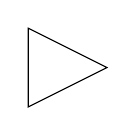
\begin{tikzpicture}[scale=0.5]
				      % Triángulo
				      \draw (2,0) -- (4,1) -- (2,2) -- cycle;
			      \end{tikzpicture}
		      }$\\
          \red{Se siente circular el pensamiento de usar la diferencia de la fórmula que tengo que probar.}

	\item la suma de los ángulos interiores de un polígono de $n$ lados es $\pi(n-2)$.
\end{enumerate}

\separador

\textit{Recurrencia}


%15
\ejercicio

%16
\ejercicio

%17
\ejercicio


\end{document}
